\documentclass[tikz,border=2pt]{standalone}
\usepackage{amsmath,amssymb}
\usetikzlibrary{arrows.meta}
\begin{document}
% (s,S) = (2,8) policy, lead time l = 1, demands 2,3,1,4,0,3,2,5,1,2: inventory level I (start value on
% the left half of each period, end value on the right half). Replenishments arrive at the starts of
% periods 5, 8 and 10, closing cycles that end in periods 4, 7 and 9 with I_4' = -2, I_7' = -1, I_9' = 0.
% Only the third cycle ends without backlog: cycle service level 1/3.
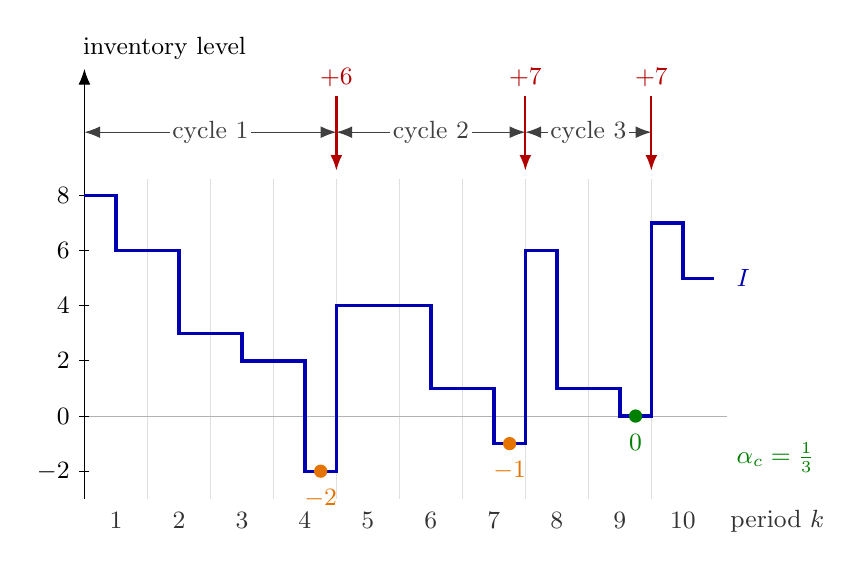
\begin{tikzpicture}[font=\small, >={Latex[length=2mm]}, x=0.8cm, y=0.35cm]
  \foreach \k in {1,...,9} {\draw[gray!25] (\k,-3) -- (\k,8.6);}
  \draw[gray!60] (0,0) -- (10.2,0);
  \draw[->] (0,-3) -- (0,12.6) node[anchor=south west, xshift=-4pt] {inventory level};
  \foreach \v in {-2,0,2,4,6,8} {\draw (0.08,\v) -- (-0.08,\v) node[left] {$\v$};}
  \foreach \k in {1,...,10} {\node[gray!40!black] at (\k-0.5,-3.8) {$\k$};}
  \node[gray!40!black, anchor=west] at (10.1,-3.8) {period $k$};
  % cycles between replenishments
  \foreach \a/\b/\n in {0/4/1,4/7/2,7/9/3} {\draw[gray!50!black, <->] (\a,10.3) -- (\b,10.3) node[midway, fill=white, inner sep=1pt] {cycle $\n$};}
  % inventory level
  \draw[blue!70!black, very thick] (0,8) -- (0.5,8) -- (0.5,6) -- (1,6) -- (1.5,6) -- (1.5,3) -- (2,3) -- (2.5,3) -- (2.5,2) -- (3,2) -- (3.5,2) -- (3.5,-2) -- (4,-2) -- (4,4) -- (4.5,4) -- (5,4) -- (5.5,4) -- (5.5,1) -- (6,1) -- (6.5,1) -- (6.5,-1) -- (7,-1) -- (7,6) -- (7.5,6) -- (7.5,1) -- (8,1) -- (8.5,1) -- (8.5,0) -- (9,0) -- (9,7) -- (9.5,7) -- (9.5,5) -- (10,5);
  \node[blue!70!black, anchor=west] at (10.2,5) {$I$};
  % replenishment arrivals
  \foreach \x/\q in {4/6,7/7,9/7} {\draw[red!70!black, ->, thick] (\x,11.6) -- (\x,8.9); \node[red!70!black, anchor=south] at (\x,11.6) {$+\q$};}
  % level just before each arrival
  \fill[orange!90!black] (3.75,-2) circle (2.4pt);
  \fill[orange!90!black] (6.75,-1) circle (2.4pt);
  \fill[green!50!black] (8.75,0) circle (2.4pt);
  \node[orange!90!black, anchor=north] at (3.75,-2.3) {$-2$};
  \node[orange!90!black, anchor=north] at (6.75,-1.3) {$-1$};
  \node[green!50!black, anchor=north] at (8.75,-0.3) {$0$};
  \node[green!50!black, anchor=west] at (10.2,-1.5) {$\alpha_c=\frac{1}{3}$};
\end{tikzpicture}
\end{document}
